\section{Diskussion der Ergebnisse}
\subsection{Energiespektren}
Während der Hintergrundmessung (Abb. \ref{untergrund}) viel nach dem ersten Peak, welcher durch die Messtechnik erklärbar ist, ein weiterer Peak mit der Spitze bei Kanal $4133.4\pm1.3$ erkennbar (Abb. \ref{untergrund_peak}).
\begin{figure}[h]
	\centering
	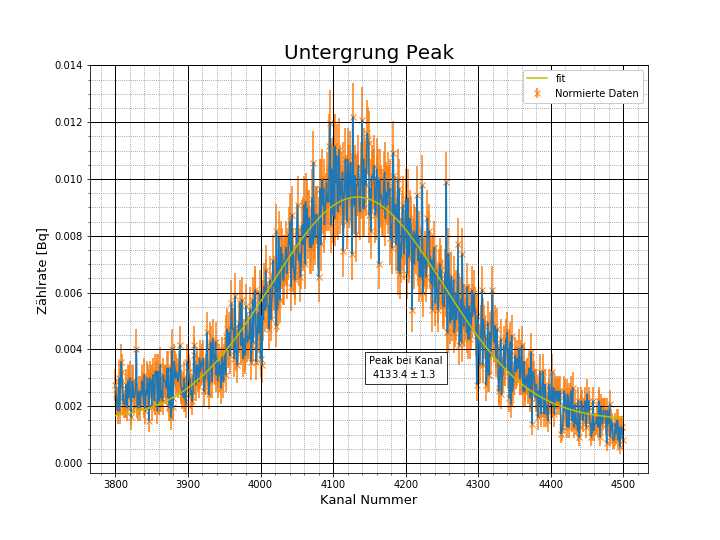
\includegraphics[scale=0.5]{Bilder/untergrund_peak}
	\caption[Peak im Hintergrund]{\small Im Bild ist der Peak im  Hintergrund Datensatz, dessen Fit und der Mittelpunkt des Fits zu sehen. Es wurde die Zählrate pro Kanal aufgetragen.}
	\label{untergrund_peak}
\end{figure}
Der Kanal im Peak wurde nach Gleichung \ref{energie-kanal} in den Kalibrierten Energiewert von $1463 \pm 6\,$keV, was in der Nähe des Übergangs von $^{40}K$ zu $^{40}Ca$ mit 1312.1 keV \cite{staatsex_szinti}. Nach der Formel \ref{vertrag} liegen diese jedoch bei einer Kompatibilität von 25 Standartabweichungen. Dies legt nahe, dass es sich um einen anderen Zefall handeln sollte. Dennoch ist dies die einzige Theorie, welche wir haben da alle im Versuch verwendeten Proben während der Messung stark abgeschirmt waren. Die Kalium Probe jedoch ist ein Pulver, welches im Versuch Lange Halbwertszeiten verwendet wird, welcher sich in räumlicher Nähe zum Versuchsaufbau befindet.\par
\begin{equation}
t = \frac{\left|x-y\right|}{\Delta_x}
\label{vertrag}
\end{equation}
Die Fits zu den Kalibriermessungen liefen Problemlos, die Resultierende Energieeichung des MCA lief auch gut, was am hohen $\chi^2$ Wert erkennbar ist.\par
Bei der Analyse des Thorium Spektrums fiel jedoch auf, dass obwohl der Fit zum jeweiligen Peak optisch nicht sehr gut passte, der Fehler auf den Parameter zum Maximum relativ klein war.
Bei der Zuordnung von den gefitteten Peaks zu den Übergängen der Thorium Zerfallsreihe viel auf, dass sehr viele Übergänge möglich waren, jedoch die meisten relativ unwahrscheinlich. Es ist dennoch nicht auszuschließen dass die gemessenen Übergänge durch zusätzlich die unwahrscheinlicheren Übergänge enthalten. Eine Analyse der 10 gefitteten Peaks des Thorium Spektrums mittels der Formel \ref{vertrag} ist in Tabelle \ref{Ergebnisse} zu erkennen.
\begin{table}
	\caption[Ergebnisse des Thorium Spektrums]{Die ermittelten Werte der Peaks des Thorium Spektrums sowie die Energien der zugeordneten Übergänge und deren Kompatibilität wurden in der nachfolgenden Tabelle aufgetragen.}
	\begin{tabular}{llll}
		\toprule
		{} & Gemessene Werte [keV] & Literaturwerte [keV] &                         Verträglichkeit \\
		\midrule
		Peak 1   &                80+/-5 &               84.373 &                                  0.8746 \\
		Peak 2   &               150+/-5 &    (131.612, 166.41) &  (3.7, 3.3) \\
		Peak 3.1 &           238.0+/-2.0 &              238.632 &                                   0.316 \\
		Peak 3.2 &           270.0+/-1.0 &               277.37 &                                    7.37 \\
		Peak 4   &           350.0+/-3.0 &               327.94 &                                 7.35333 \\
		Peak 5   &           410.0+/-2.0 &               415.27 &                                   2.635 \\
		Peak 6   &               519+/-5 &                510.7 &                                    1.66 \\
		Peak 7   &               591+/-5 &                587.8 &                                    0.64 \\
		Peak 8   &               839+/-5 &                835.9 &                                    0.62 \\
		Peak 9   &             2614+/-10 &              2614.51 &                                  0.0511 \\
		\bottomrule
	\end{tabular}
\label{Ergebnisse}
\end{table}
Es ist erkennbar, dass einige Werte relativ nahe an den Entsprechenden Literaturwerten liegen, andere jedoch weit von ihnen entfernt liegen. Dies ist insbesondere bei den Peaks 4 und 5 der Fall. Dies kann zum Teil durch Überlagerung von Comptoneffekten der darauffolgenden Peaks erklärt werden. Zusätzlich ist es sehr auffällig, dass die geschätzten Fehler groß sind, sodass die gemessenen Peaks teilweise sehr kleine Inkompatibilität haben. Dies ist vor allem bei Peak 9 der Fall, wo der gemessene Wert mit dem Literaturwert fast vollends übereinstimmt. 
\subsection{Winkelabhängige Messung}
Auch hier wurde die Kompatiblität des gemessenen Wertes von $-0.81\pm0.11\,$Grad mit dem erwarteten Wert von $0^\circ$ über die Formel \ref{vertrag} verglichen mit dem Ergebnis 7.4, wonach sie nicht kompatibel sind. Bei Betrachtung der Abbildung \ref{Winkelbild} fällt auf, dass im wichtigen Bereich die Datenpunkte vom Fit stark abweichen. Daraus kann man folgern, dass dieser Fit nicht repräsentativ für die Daten der Wichtigen Region ist. Bei Betrachtung der Daten einzeln fällt auf, dass mit Abstand die höchste Anzahl an Counts bei $0^\circ$ gemessen wurde, was darauf hinweist dass ein Problem mit dem Fit vorliegt.